This chapter illustrates the system architecture and describes the role of each component.
It also contains an analysis of why the architecture is scalable.

The system architecture is introduced to ease maintenance and ensure scalability.
The architecture consists of four macro components and a database, as can be seen in \Cref{fig:architecture}. The macro components are: Shared, Location Service, Model Agent, and Web Service.

\begin{figure}
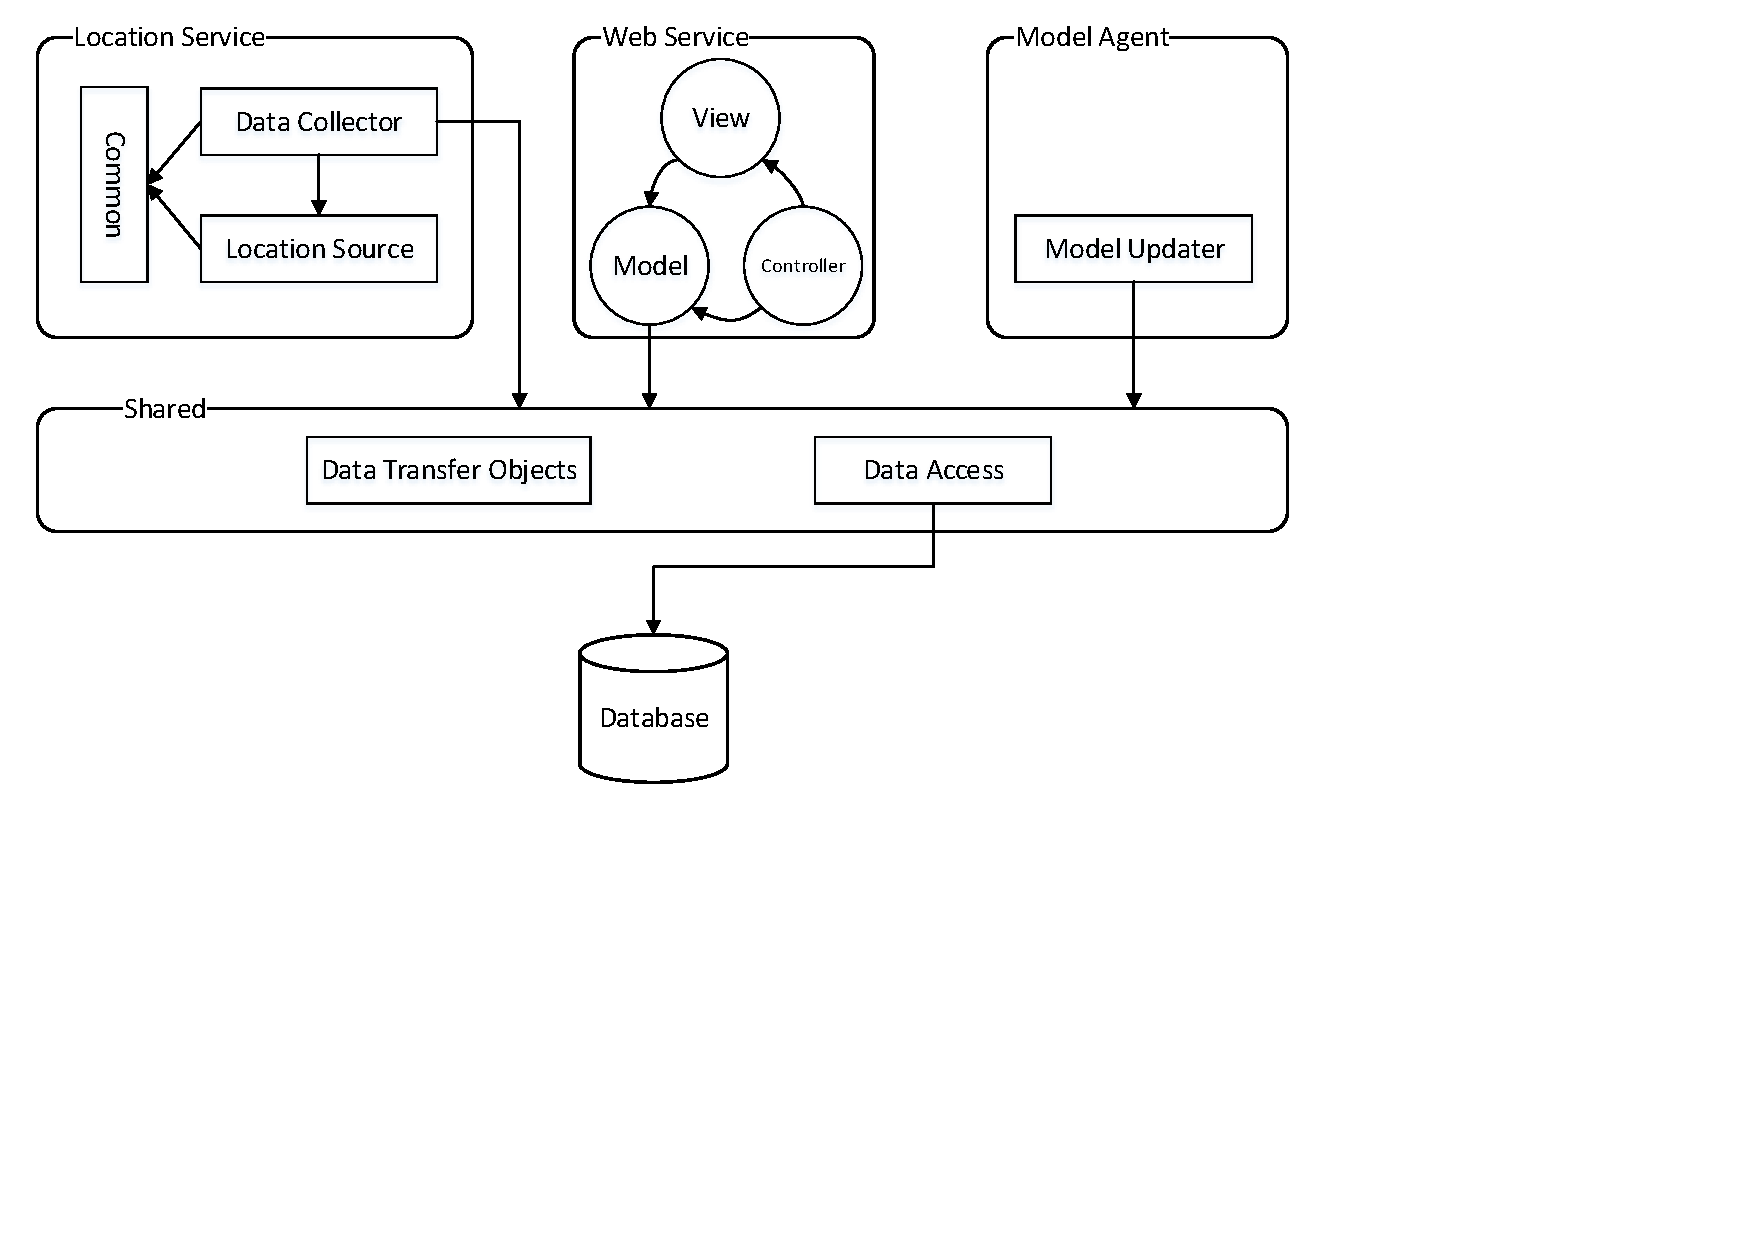
\includegraphics[width=\textwidth, trim={2cm 1cm 6cm 0}]{systemArchitecture.pdf}
\caption{The architecture of the system}
\label{fig:architecture}
\end{figure}

\section{Database} The database used is a MySQL database, and is where all our data is stored.
The design of the database can be found in \Cref{database_design}.
It is not included in the report as its structure is rather trivial and only serves the purpose of having a simple and fast method of storing/retrieving large amounts of data.

\section{Shared}
The task of the shared macro component is to provide extended capabilities to all other macro components.
The component provides a shared structural representation of data and a uniform set of database connection methods.

\paragraph{Data Access} All SQL statements and communication with the database are encapsulated here providing the upper layers a communication protocol to the database.
Additionally this layer provides an abstraction of the actual communication with the database as well as an abstraction of the database design.

\paragraph{Data Transfer Object} This layer provides a collection of shared data types, making it possible for all the macro components to treat the data uniformly.
The types within this layer provides methods for retrieving data from the database and converting it into elements of the types in the Data Transfer Object layer.

\section{Location Service} 
The location service component processes and stores location data directly from a data source.
In other words it serves the purpose of loading gps location data for the other components (through the shared macro component).

\paragraph{Location Source} Provides an implementation of a data-source from which data can be retrieved.
The common layer in provides a shared structure for communication between the location layers.

The layer is structured such that the Location Source layer can easily be replaced with another source of data\footnote{This is used for providing data when testing the system, as will be described in \cref{design:datasimulation}.}.

\paragraph{Data Collector} Using a data source defined in the location source layer, this layer gathers the gps location data and stores it in the database using the shared macro component.

\section[title]{Model Agent\footnote{An agent is defined as a program that invoke a given task, when a condition is satisfied, then returning to a sleeping state, until the condition is satisfied again.\cite{definitionagent}}}
The task of the model agent macro component is to generate and update the hotspot and Markov chain model in the database (through the shared macro component).

\paragraph{Model Updater layer} This is where the generation of the model is handled, which works as follows:\\
Clusters are created based on the GPS data in the database.
This is done using DBSCAN, as described in \Cref{clustering:DBSCAN}.
The convex hull of each cluster is determined, by using Graham Scan, and these are saved to be used as hotspots.
The Markov chain matrix is now created with these hotspots, and their departures, as was described in \Cref{markov:create_model}.

Finally, since we have no further use of it, all already modelled GPS data is truncated from the database, with exception of the single latest location of all bikes.

\section{Web Service}\label{arch:webservice}
Web Service is the macro component containing a Model, View, and Controller.
The task of the macro component is to provide a web service, in order for users to interact with the system.
The model, view, and controller of the web service were introduced in \Cref{webapi:mvc}.
